A primeira fase é destinada a definir o plano de ação que deve ser seguido durante o restante do processo. Todas as atividades desta fase são realizadas pelo Iniciador, que é quem define as características do objeto de aprendizagem a ser gerado, e do processo de colaboração.

\begin{figure}[ht]
\centering
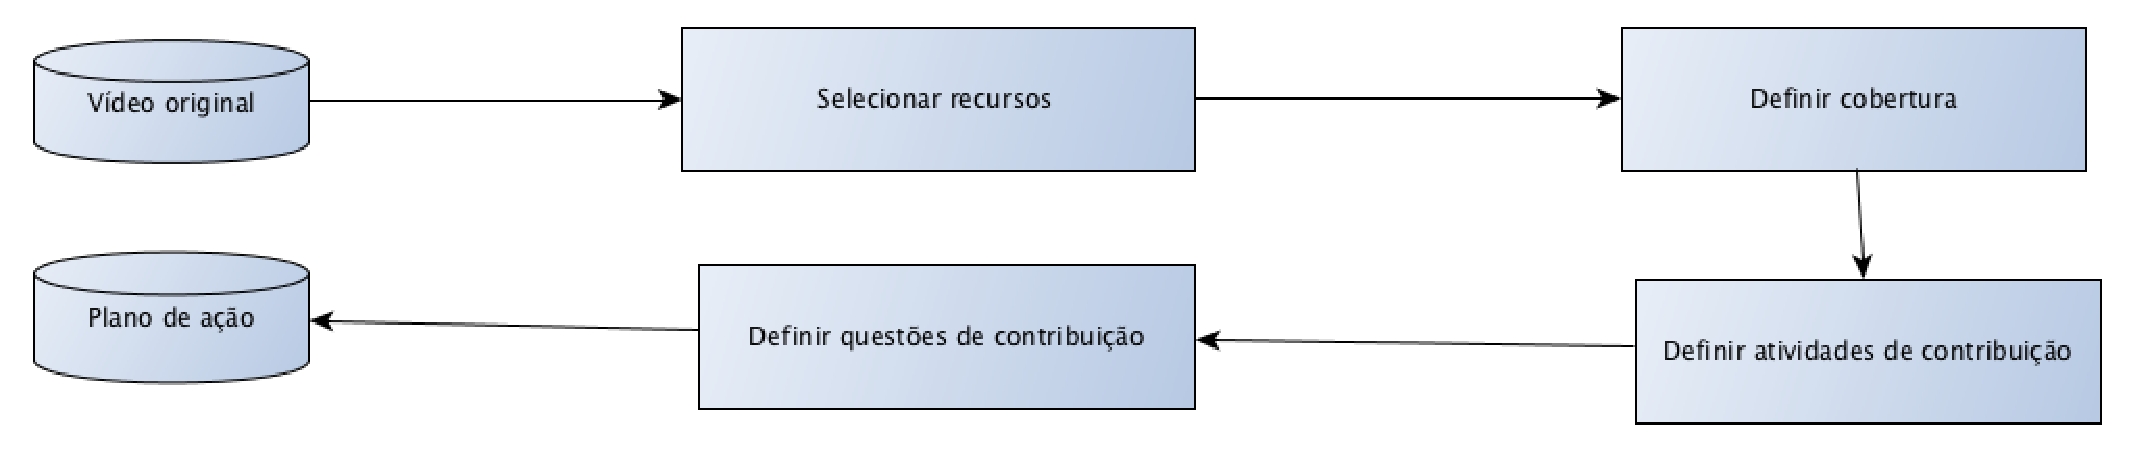
\includegraphics[width=.99\textwidth]{imagens/metodo/fase1_oa.eps}
\caption{Fase 1 do método}
\label{fig:metodo:fase1}
\end{figure}

Como pode ser observado na Figura~\ref{fig:metodo:fase1}, esta fase tem inicio com a seleção de quais são os recursos e tipos de conteúdo que serão agregados ao vídeo. Este método suporta qualquer recurso que possa ser agregado ao vídeo, ou apresentado coerentemente com ele, desde sumários, controles aprimorados e representações em Libras (Língua Brasileira de Sinais), até imagens, fontes de áudio e mapas de navegação. Todavia, por questões de escopo, foram selecionados três recursos para serem utilizados neste trabalho: imagens, caixas de texto, e hiperlinks. De modo geral, o que limita os recursos utilizados não é o método, mas o ambiente que será utilizado, pois é necessário implementar suporte para cada um deles.

Após determinar o que será agregado ao vídeo, o Iniciador precisa definir quais são os pontos que deseja cobrir, ao definir a cobertura é possível distribuir as tarefas entre os estudantes para obter as informações necessárias. Uma vez definida a cobertura, devem ser selecionadas quais são as atividades que devem ser realizadas pelos estudantes. Uma das contribuições deste trabalho é padronizar as atividades pelas quais se pode contribuir com o processo. Estas atividades são modeladas como tarefas de anotação, de forma que foi possível definir três tipos de atividade de contribuição: identificar lacunas semânticas, sugerir conteúdo para preenche-las, e avaliar sugestões de conteúdo dos outros estudantes. O Iniciador deve selecionar quais delas devem ser realizadas pelos estudantes. 

Por fim, o Iniciador deve configurar as questões de contribuição, que irão orientar os estudantes sobre como deve realizar as atividades, e de que forma devem contribuir. Todas estas definições são então compiladas em um plano de ação que guiara todo o processo.







